 %%%%%%%%%%%%%%%%%%%%%%
\section{Numerical Experiments}
\label{sec:NumExp}

For our numerical experiments, we aimed to extract qualitative features of both small, toy networks, as well as of larger workhorse networks suitable for use on real world tasks (e.g. MNIST).  At its core, the maximum interpolated error (i.e., \eqref{eq:minmaxerror}) is a measure of problem nonconvexity---or, more precisely, of the nonconvexity of the loss surface of a given architecture on a particular learning problem.


\subsection{Polynomial Regression}
\label{sec:PolyFuncs}
%%%%%%%%%%%%%%%%%%%%%%

 Polynomial function regression is a task for which small neural networks can achieve extremely high accuracy.  For our numerical experiments, we studied a 1-4-4-1 fully connected multilayer perceptron style architecture with RELU activation and RMSProp optimization.  For ease-of-analysis, we restricted the family of polynomials to be strictly contained in the interval $x\in[0,1]$ and $f(x)\in[0,1]$.
 
 Discussion of different Loss functions
 
 etc.


%%%%%%%%%%%%%%%%%%%%%%
\subsection{Convolutional Neural Networks}
\label{sec:CNN}
%%%%%%%%%%%%%%%%%%%%%%



%Exploitation
\begin{figure}
\label{figurelength}
\centering
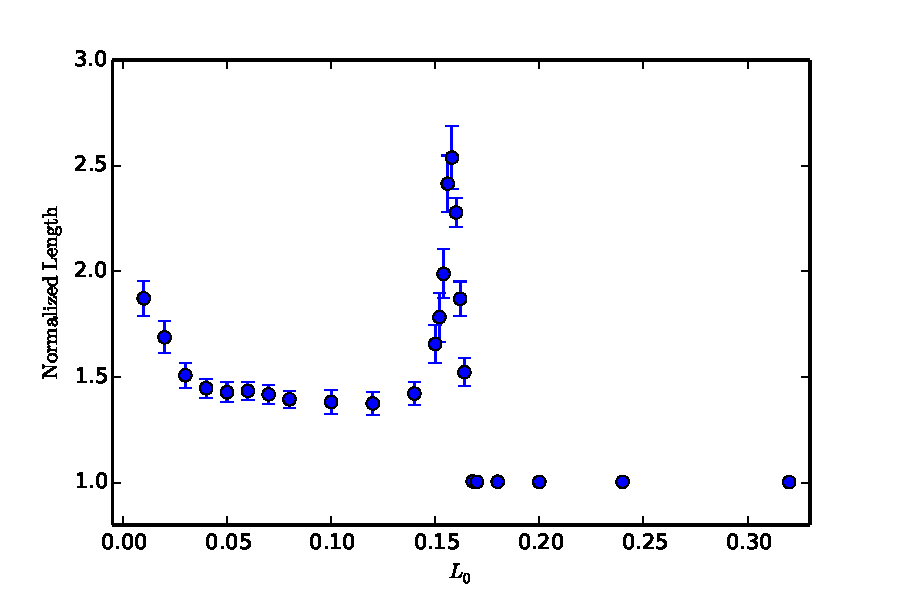
\includegraphics[width=.4\textwidth]{../Plots/normlengthcubics}
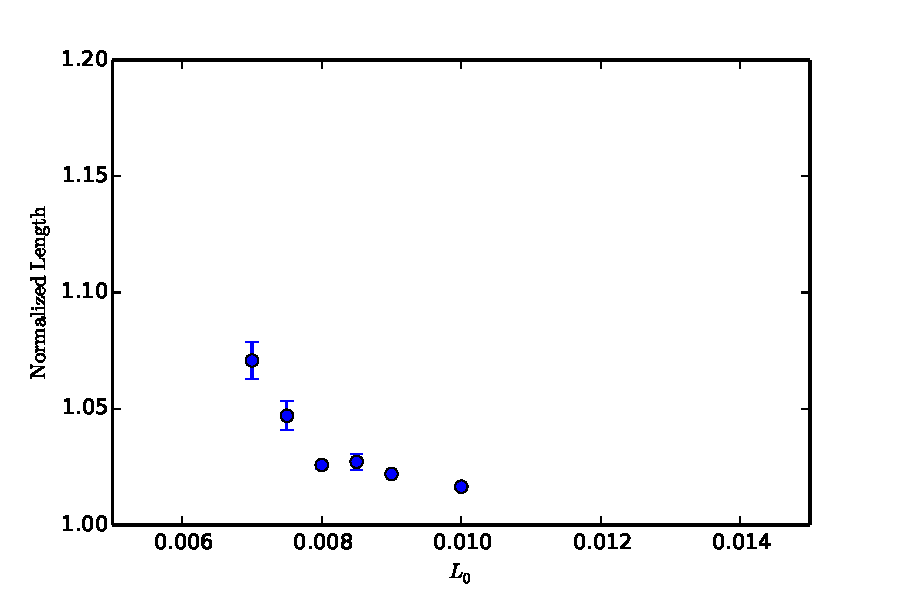
\includegraphics[width=.4\textwidth]{../Plots/normlengthMNIST}
\caption{Normalized geodesic length as a function of the energy level for two different models. Left: a ``low-dimensional" neural network 
attempting to fit a cubic polynomial. Right: a convolutional neural network on MNIST. Whereas the cubic fitting displays a heavily non-convex structure 
at mid-energy values, the MNIST example qualitatively behaves as a convex loss, in which geodesics approach straight lines.}
\end{figure}

\subsection{Recurrent Neural Networks}


